\def\DevnagVersion{2.17}\documentclass{article}
\usepackage[utf8]{inputenc}
\usepackage{graphicx}
\usepackage{subcaption}
\usepackage[a4paper, total={170mm,257mm}, left=25mm, top=20mm, right=25mm, bottom=20mm]{geometry}
\usepackage{indentfirst}
\usepackage{soul}
\usepackage{float}
\usepackage{enumitem}
\usepackage{devanagari}
\usepackage[colorlinks=true, linkcolor=blue, urlcolor=cyan]{hyperref}

\title{An Extensive Study of the Cheems Language}
\author{Sayam Sethi (2019CS10399)\\Shrey Patel (2019CS10400)\\Rishi Shah (2019CS10394)}
\date{November, 2021}

\begin{document}

\maketitle

\tableofcontents

\newpage

\begin{abstract}
    Nowadays, memes are very popular throughout the Internet. They are used to express feelings, like happiness, anger, or sadness. They have become one of the most dominant forms of communication in the digital age and possibly the most favourite pastime of the younger generation. The beauty of a meme is that it is not just a picture, but a story. The story is the main content of the meme, and the story is the main reason for the popularity of the meme. And another feature of memes, that results from the larger context of the memes,  is that more often than not, they are interpreted differently by different people. Due to this, sometimes, even a single meme, which is nothing more than a piece of image or text, becomes a recurrent topic of discussion, as evident from the thousands of comments following some of the more popular memes on Reddit or Instagram.

    Following this reasoning, we will try and analyze the effect memes have on language. We use the meme language \textbf{Cheems} for our case study. We intend to delve deep in the origin, history, and usage of the language and also try to understand the usage of the language in the context of the memes. We will also discuss the evolution of the language among the community using various conversational examples and try to put forth various opinions of different language groups on the validity of the language.

    The above discussion is significant because it reflects on the development of languages in short term, and highlights the importance of digital media in this day and age and the impact it has shown on our community as a whole. We will try to show that the technology of today has played a pivotal role in truly turning the world into a global village, and we speculate that this study will give us an insight on the future development of languages or atleast what we can expect going forward.
\end{abstract}

\section{Theoretical Framework}

\subsection{Introduction}

\subsubsection{A traditional language}
Normally, a particular language develops and evolves over hundreds and possibly thousands of years, for it to seep through a wide and diverse range of language communities. Most of the traditional languages like Hindi, Gujarati, English, etc. have been spread and passed upon, more or less through direct human communication and have been used in the past for a long time.  The prevalence which these languages have achieved is primarily because it has been passed and propogated through a variety of media like human speech and interaction, writing in the form of print media. But note that the biggest hindrance to the rapid spread of these languages is the sense of locality. The geographical barriers have caused the language spread to be abysmally slow and gradual.

\subsubsection{A ``Meme'' language}
However, the digital media today has caused information to flow much faster, regardless of barriers. So, nowadays, people are quicker to adapt to various cultural (especially related to language) and technological trends and concepts as compared to the past. People today are much more likely to be aware of affairs and incidents happening in different parts of the world. The teenagers today use a whole array of web jargon which supposedly makes them appear ``cool'' among their peers, like \textit{lol} (laugh out loud), \textit{gg} (good game), \textit{brb} (be right back) and so on. And what's fascinating is that all these web jargon then becomes a part of their daily language as well. It is not uncommon to come across who prefers to actually speak \textit{lol} instead of actually laughing at some joke or humorous remark. Another surprising fact about these internet ``lingo'' (pun totally intended) is that its users don't actually go through any sort of training or learning process. It's just practice through usage. No rules, no bounds, only usage. The surprising fluency may be because these are generally derived from a parent language, mostly English, but may be extended to other languages as well or due to the fact that the users of this language are quite frequently exposed to the usage of this kind of abbreviated language in different parts of the net. The constant exposure seems to be the better reason for the rapid growth in its users.

Memes play a kind of a unique role in propogating this information. One might ask that online educational portals, blogs or research papers that are freely available throughtout the Internet should be the primary sources of intellectual ideas and concepts, and they are, to a large extent, but the painful reality is that most of us are often not patient or curious enough to dig through scores of \st{bland} text to get our daily dose of brain food. Most of us won't even log onto the Internet intending to learn something new but just to have fun or kill some time. Memes come to rescue in this scenario. They are fun, witty, and informative (mostly). Many times, they mock some stereotyped belief using hilarious examples or situations, or depict raging and controversial topics in a light-hearted manner.

But the general view among the \st{boomers} digitally innocent generation is that the memes are a useless waste of time, that fill the brain with twisted and unconventional ideals and that they are another one of those undesirable outcomes when you give the youngsters too much freedom of speech and expression. But, memes are much more than just mere social media posts, they are a part of the digital culture. Let's take an example. Consider the following meme:

\begin{figure}[H]
    \centering
    
\includegraphics[width=0.4\textwidth]{figures/meme1.png}
    \caption{A typical Internet meme}
\end{figure}

Now, the above meme has two visible humorous elements. One is exploiting the similarity between the spellings of ac-tor and doc-tor to create a sense of contrast. And the other, more intellectual one, is the satire on Indian education in which the meme refers to the situation in which a child conveys his dream/wish of becoming an actor to his father, but the stereotypical Indian father only considers being a doctor (or an engineer :) ) to be a good job, since they are usually the most respected/highly paid jobs in the country. So, in a satirical way, this meme portrays the state of Indian education and economy, though exaggerated, to the rest of the world, since the Indian culture has historically been the one which glorifies hard work, skill, progress and innovation. However, this doesn't mean that the Indian culture has ever undermined or ignored talents in other fields like art, music, design, etc.

Now, in the rest of the paper, we will look at a particular meme which took the world by storm (kind of). It is one of those memes whose study is very valuable from a linguistic point of view. We will look at the "Cheems" meme.

\subsection{Origin and Etymology of Cheems}
Before \textbf{Cheems} became famous, a certain set of memes called \textbf{doge memes} rose to prominence. The word \textbf{doge} is a misspelling of the word \textit{dog}. One of the initial versions of the meme is:
\begin{figure}[H]
    \centering
    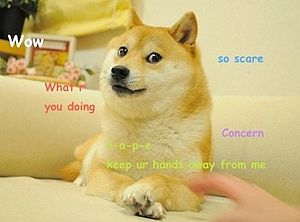
\includegraphics[width=0.5\textwidth]{figures/original_doge_meme.jpg}
    \caption{Original Doge Meme}
\end{figure}

As can be clearly seen from the meme, even though the language is still English, the way the phrases are structured gives it a very different feeling. Additionally, the phrases are terse and they don't follow the regular English grammar. In a way, the words use their root form instead of using the contextual morphemes. Another example of a meme of this category is:
\begin{figure}[H]
    \centering
    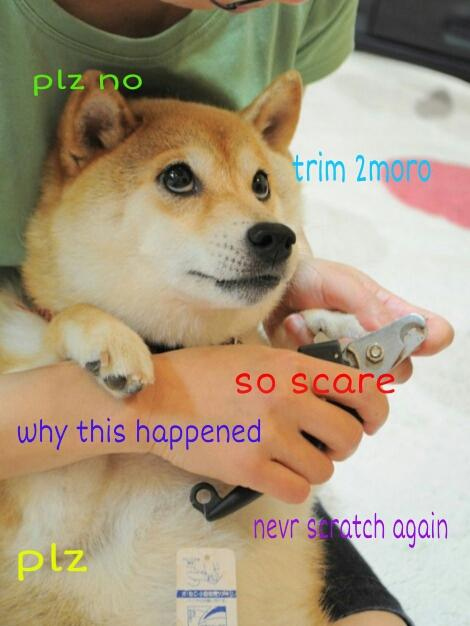
\includegraphics[width=0.3\textwidth]{figures/doge_2.jpg}
    \caption{Another example of the \textit{doge meme}}
\end{figure}

Again as we can see, the meme aims to convey a story without using too many words and it has the \textit{doge} flavour of English. The story being narrated is as follows:
\begin{itemize}
    \item The dog is requesting its master to not do something
    \item We then find out that the dog is requesting the master to trim its nails the next day
    \item The dog conveys that it is scared
    \item They also wonder why the master has decided to trim their nails
    \item They conclude that the master is trimming their nails because they scratched someone and hence promise that they will never scratch again
    \item The meme then ends with the dog requesting again
\end{itemize}


\subsubsection{Origin of the Doge Dog}
The dog in the original meme has been traced back to a female dog of the breed \textit{Shiba Inu} called \textbf{Kabosu}. On February 13th, 2010, Japanese kindergarten teacher Atsuko Sato posted several photos of her rescue-adopted Shiba Inu dog Kabosu to her personal blog. Among the photos included a peculiar shot of Kabosu sitting on a couch while glaring sideways at the camera with raised eyebrows. This is how the stock meme image originated. The first meme came to light in July 2013. The meme then went on to become the top meme of 2013 by \textbf{Know Your Meme}.\\
The popularity of the doge meme also led to creation of a cryptocurrency being named \textbf{Dogecoin}. The cryptocurrency was created by a team of developers who were inspired by the doge meme. \textbf{Dogecoin} was officially launched on December 6, 2013.
\begin{figure}[H]
    \centering
    
\includegraphics[width=0.3\textwidth]{figures/Dogecoin_logo.png}
    \caption{Dogecoin Logo}
\end{figure}

\subsubsection{Shift from Doge to Cheems}
Since the introduction of the Doge meme, there have been various spin-offs and \textbf{Cheems} is one of them. On September 4th, 2017, Instagram user \href{https://www.instagram.com/balltze}{@balltze} posted an image of a Shiba Inu. The image of the dog's head was later used in ``Cheems'' memes. The earliest known usage of ``Cheemsburbger'' was published on the /r/dogelore subreddit on June 8th, 2019. This is what inspired the name \textbf{Cheems} and the language of `m'. One of the initial meme is presented here:
\begin{figure}[H]
    \centering
    
\includegraphics[width=0.4\textwidth]{figures/cheems_1.jpg}
    \caption{One of the first Cheems meme hinting at the modified language}
\end{figure}

The meme further evolved into the \textbf{Buff Doge vs. Cheems} meme in which representatives of the same group from two historical eras are presented as Swole Doge and Cheems and are compared to each other. One such meme is as follows:
\begin{figure}[H]
    \centering
    \begin{subfigure}{0.45\textwidth}
        \centering
        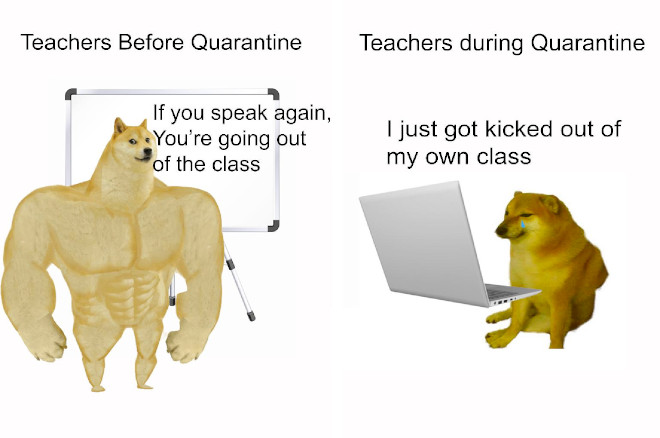
\includegraphics[width=\textwidth]{figures/cheems_2.jpg}
    \end{subfigure}
    \begin{subfigure}{0.45\textwidth}
        \centering
        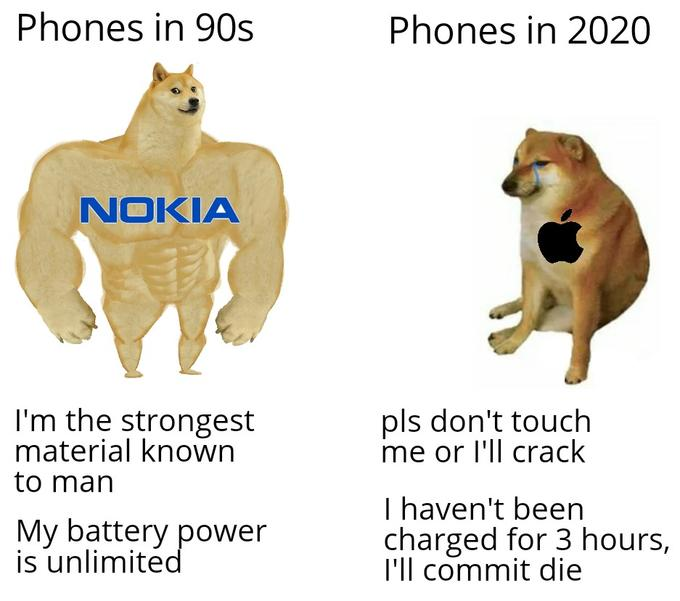
\includegraphics[width=0.7\textwidth]{figures/cheems_3.jpg}
    \end{subfigure}
    \caption{Couple of examples of ``Buff Doge vs Cheems'' meme}
\end{figure}

As can be seen, this meme depicts the generation gap and the shift from the \textit{Doge} to the \textit{Cheems} generation. Most memes similar to this one, aim to show the increase in the \textit{luxurious} lifestyle of the people with time and hence they have become \textit{weaker} and highly dependent on the excessive amenities given to them. Additionally, they show how the newer generation has become less tolerant to the various adversities in life and hence they are more prone to depression and anxiety.

\subsection{Transition from Meme to Language}
As we mentioned above, the Cheems language started as a meme and as we might assume in normal circumstances, memes are generally free-form, in the sense that they don't follow any pre-determined structure or grammar rules, while on the other hand, any widely spoken language (however arbitrary) tends to follow some rules or basic structure, some of which are decided by common universal logic (on the basis of pronounciation, meaning, etc.), while othe rules may be enforced implicitly by persistent usage. We present some of those rules here. However, note that most of these rules are not concrete, since they are based on observations and experiences of usage of this language.\par
Cheems is an infant language which initially started with a few fun-sounding words like \textit{dom't, birmd, thamk}, etc. It's not difficult to notice that all of these words are derived from English words by adding the letter 'm' at appropriate places. This is the only rule which is concrete, since it is the identity of the language itself. All the other rules that we list next are speculations based on observations.

\subsubsection{Rules for adding ``m''}
\begin{itemize}
    \item The letter ``m'' is usually added (if added) in the coda of any particular syllable of the corresponsing English word. And most of the times, it is added right after the vowel of the nucleus, as in $bad \to bamd$, where the letter ``m'' is added after the vowel ``a'' in the coda ``md''.

    \item In cases where the coda has multiple potential places of insertion, like in \textit{bird}, the place of insertion of ``m'' depends upon how much sense the resulting pronounciation makes after adding ``m''. For example, pronouncing ``birmd'' is easier than pronouncing ``bimrd'' or ``birdm''.
          \begin{figure}[H]
              \centering
              \begin{subfigure}{0.45\textwidth}
                  \centering
                  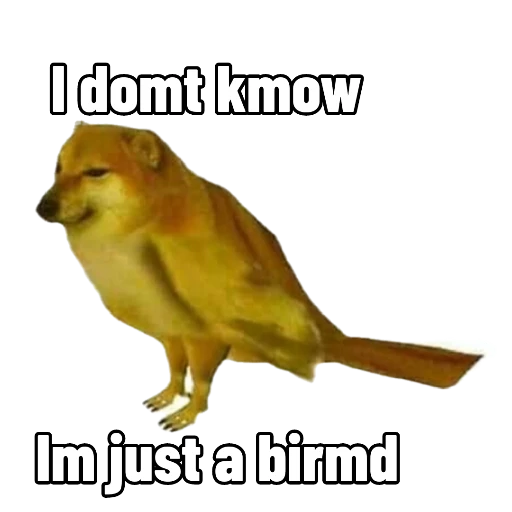
\includegraphics[width=0.66\textwidth]{figures/birmdie.png}
              \end{subfigure}
              \begin{subfigure}{0.45\textwidth}
                  \centering
                  
\includegraphics[width=0.66\textwidth]{figures/birmdie_hindi.png}
              \end{subfigure}
              \caption{Examples of the rules for adding ``m''}
          \end{figure}

    \item If , multiple places of insertion of ``m'' result in similar pronounciations, then we (this is a completely personal rule) use both the words in conjunction. For example, in the word \textit{yes}, we can insert ``m'' at two different places to obtain two Cheems variants of \textit{yes}, i.e. \textit{yems} by adding ``m'' before ``s'' or \textit{yesm} by adding ``m'' after ``s'' and both these words can be pronounced with same degree of ease. So, instead of using only one of them, we use \textit{yemsyesm} instead. Hilarious and out of logic, I know, but convenient.

    \item For certain words, it might be required to replace an existing letter in the word with ``m'' instead of just inserting it so as to not distort the pronounciation too much. This happens mainly in the cases where the letter ``m'' is present is the coda of a syllable, like the word \textit{sink}. It would be impossible (or atleast rather cumbersome) to pronounce \textit{sinmk}, \textit{simnk} or \textit{sinkm} without making one of ``m'' or ``m'' silent. So, we simply replace ``n'' with ``m'' to obtain \textit{simk}. Much better, right?

    \item The main problem arises when a syllable already has the letter ``m'' in it, in which case simply adding ``m'' complicates the pronounciation even more. For example, consider the word \textit{swim}. The letter ``m'' is coda itself in this single syllable word. So, adding ``m'' to coda to obtain \textit{swimm} doesn't change much to the pronounciation at all. So, we don't add another ``m'' and keep the word as it is.

    \item Additionally, there is a scope of adding ``m'' to the onset of any syllable as well. For example, take the word \textit{Sayam}. Our previous rules suggest that the Cheems word for Sayam will be \textit{Samyam} by adding to the coda of first syllable and keeping the second syllable unchanged. But, how about changing the onset of the first syllable instead of coda, how about \textit{Smayam}. It doesn't sound bad at all. And considering that most of these rules have only been enforced based on a handful of observed data and the usage of the language in memes, we might be in no place to reject it. The funny thing is that the second word is no harder to pronounce than the first one, so both the words fit our pronounciation criteria.

    \item But, from what we have observed so far, the coda rule seems to fit and explain many different Cheems words as compared to the onset rule, and so we will go forward considering this to be correct and any words which fit the language but not the rules above, will be considered as exceptions, since they don't fit the general trend observed till now.
\end{itemize}

As we can see, there are quite a few (although loose) rules on deciding whether a word may be a part of the Cheems language or not. At this point, these are used mostly for elimination of words that should not belong to the language as opposed to providing an exhautive one-to-one mapping of the corresponding English words, because as we mentioned, the Cheems language is itself a meme, and therefore a fundamentally open-ended concept, which can be interpreted in different ways by different language communities. Another notable feature of this language is that the main criteria in choosing or eliminating a potential candidate is the pronunciation of the word. We tend to choose that word which is the most hilarious and has easier pronounciation.

\subsubsection{Extension to other languages}
Till now, we primarily considered Cheems to be the language constructed of words derived from those of English language. But we feel that we can apply similar rules to the words of other languages like Hindi to achieve the same conversion effect. Say, for Hindi, the effect of adding ``m'' in English can be replaced by adding {\dn \qq{m}} or {\dn m} in Hindi. The same rule holds for Gujarati.

Thus, in Cheems variants of different languages can be obtained by suitably substituting ``m'' with a similar sounding character in the other language. We will call this character as the placeholder for now. The other rules regarding the position or replacement of this placeholder in the syllables of any word in the base language remain more or less the same.


\section{Examples from Data}

\subsection{Is Cheems Acceptable?}
We now attempt at reproducing an actual conversation that happened between a few hostelmates of ours (about half a year ago).
\begin{itemize}[label={}]
    \item \textit{Shrey:} Hello Sayam and Paaji. How are you doing?
    \item \textit{Samyam:} Hemlo Shmrey, I am doimg fimne.
    \item \textit{Paamji:} Yemsyesm, me too.
    \item \textit{Shrey:} What's wrong with you two? Your way of speaking makes it sound like you guys might have aphasia.
    \item \textit{Paamji:} Nompe, thims is our way of limfe. We hamve adampted to the way of Cheems.
    \item \textit{Shrey:} I don't like the way you are speaking. It makes it sound so cringe.
    \item \textit{Samyam:} Dom't womrry, I was surmprimsed by the Cheems lamguage but I hamve come to accempt it to a larmge extemt. You wimll gemt used to it too.
    \item \textit{Paamji:} Also, Cheems is vemry fumnny too. It makes such simple soumdimg wormds of Emglish become so imteremstimg.
    \item \textit{Shrey:} Well, I still can't understand what you guys are thinking. Nevertheless, it is weirdly fun to hear you guys talk like this. Continue!
\end{itemize}
And then this particular \textit{Shrey} is the same person who has now accepted the way of \textbf{Cheems} and is now writing this particular term paper on this very topic. A sample conversation involving him follows in the next subsection.

\subsection{A Random Conversation between three Cheems Users}
\begin{itemize}
    \item $Rishi \rightarrow Ri+m+shi = Rimshi$
    \item $Sayam \rightarrow Sa+m+yam = Samyam$
    \item $Shrey \rightarrow Sh+m+rey = Shmrey$
\end{itemize}
Conversion between the three peers:
\begin{itemize}[label={}]
    \item $Rimshi$: Hemlo Shmrey, how are you?
    \item $Shmrey$: Hemlo Rimshi, I am goomd. Are you in campus?
    \item $Rimshi$: Yemsyesm, I came yemsterday.
\end{itemize}
Meanwhile, Samyam joins the conversation.
\begin{itemize}[label={}]
    \item $Samyam$: Come on you gumys, aren't you forgemtting something!
    \item $Rimshi$ and $Shmrey$: Whamt?
    \item $Samyam$: We have a deamdline for the term pamper tomday. Have you even demcided the tompic yet?
    \item $Shmrey$: Yemsyesm, the term paper is for lamguage course. So why not write ambout our namtive lamguage.
    \item $Rimshi$: Shmrey, are you remferring to Cheems?
    \item $Shmrey$: Examctly!
    \item $Samyam$: Oh yeah! Cheems is not just a lamguage, its an emotion for us. Brimlliant imdea Shmrey.
    \item $Shmrey$: Thamk you, as always my imdeas are permfect.
    \item $Rimshi$: So whamt are you waimting for, lets starmt working on the paper.
\end{itemize}
A few moments later$\ldots$
\begin{itemize}[label={}]
    \item $Rimshi$: Gumys, have you starmted premparing for the mamjors?
    \item $Shmrey$: Oh Rimshi, sumch a foomlish question. You know I am emvereamdy for the majors.
    \item $Samyam$: I am yemt to start premparing. As always I will have to stumdy nimght before the majors.
    \item $Rimshi$: Yemsyesm, same here. However there's ome sumbject which I am comfident to score goomd gramdes.
    \item $Samyam$: Yeah HUL243 rimght! Just by attemding the lemctures, we get fumll clamrity of the sumbject and score goomd marks.
    \item $Shmrey$: Yemsyesm, it is also one of my famvourite sumbject.
\end{itemize}
One minute before the submission deamdline.
\begin{itemize}[label={}]
    \item $Shmrey$: Humrray! We dimd it.
    \item $Samyam$: Umff agaim a lamst minute submimssion.
    \item $Rimshi$: Yemyesm, thats the stomry of our comllege. We do emverything in the lamst momements.
    \item All Together: Amll is wemll that emds wemll.
\end{itemize}

\subsection{Cheems on the Internet}
There are numerous places the \textbf{Cheems} culture is prevalent on the internet. \href{https://www.reddit.com}{Reddit} and \href{https://www.4chan.org}{4chan} are two of the most popular places. On \textbf{Reddit}, the \textit{subreddit} \href{https://www.reddit.com/r/dogelore}{r/dogelore} is a thriving community with over $325k$ subscribers and about $1.4k$ people online at the time of writing this paper. A very recent meme which is on \textit{hot} is the following:
\begin{figure}[H]
    \centering
    \begin{subfigure}{0.45\textwidth}
        \centering
        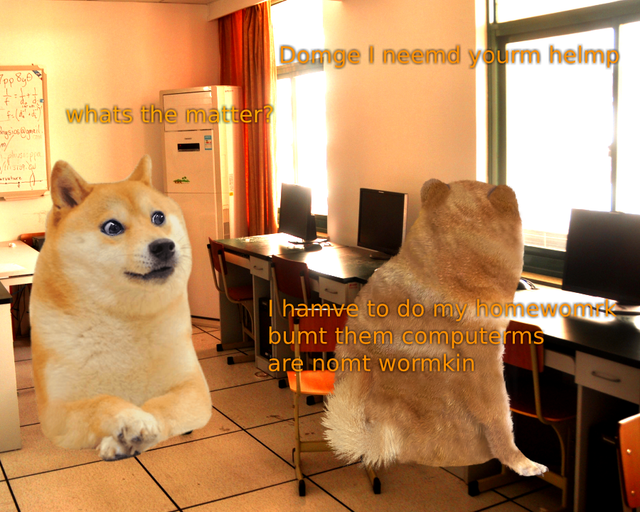
\includegraphics[width=0.9\textwidth]{figures/reddit_1.png}
    \end{subfigure}
    \begin{subfigure}{0.45\textwidth}
        \centering
        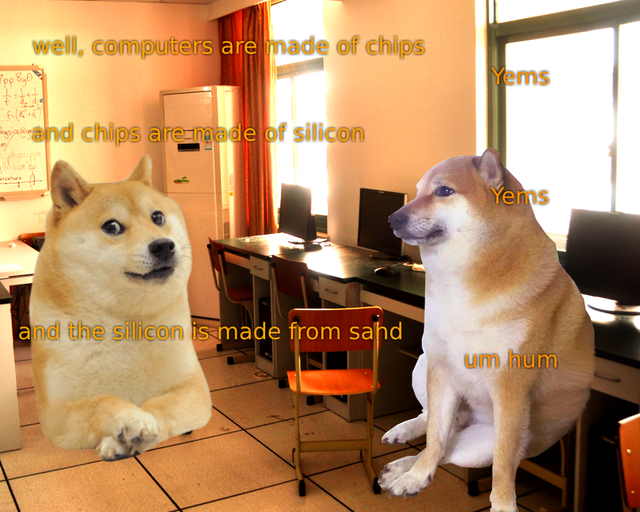
\includegraphics[width=0.9\textwidth]{figures/reddit_2.png}
    \end{subfigure}
    \caption{First two panels of a meme taken from r/dogelore}
\end{figure}

Apart from \href{https://www.reddit.com/r/dogelore}{r/dogelore}, there are atleast about $5-10$ memes every day related to the \textit{Cheems} format on the following subreddits:
\begin{itemize}
    \item \href{https://www.reddit.com/r/memes}{r/memes}
    \item \href{https://www.reddit.com/r/dankmemes}{r/dankmemes}
    \item \href{https://www.reddit.com/r/meme}{r/meme}
    \item \href{https://www.reddit.com/com/r/memeeconomy}{r/MemeEconomy}
    \item \href{https://www.reddit.com/r/Me_irl}{r/Me\_irl}
\end{itemize}

Additionally, there is also a website which is used to convert English speech to \textbf{Cheems}. The website is \href{https://cheems.mirazmac.com/}{Cheems Translator} and on exploring, it was found that the developer of the website is a programmer (from the GitHub page of theirs). However, the source code of the website hasn't been made public so we could not actually analyse the actual syntax used for translation. However, from experimentation with different phrases on the website we have concluded that most of the syntactic conversions are consistent with the rules that we have stated above. Therefore, the language has a consistent terminology that everyone across the world agrees on.

\section{Problems of Fit}

We identify the following three \textbf{A's} as the problems of fit:

\subsection{Acceptance}
As evident from the mock discussions and conversations we mentioned, the acceptance of the language as a valid form of expression and communication is debated as we can see from the above two types of conversations, as many consider it to be an extension of an immature joke/meme taken from the Internet. So, there is no clear consensus on the usage of this language and therefore it may be a bit difficult to discuss the development of this language in border language communities of the world, although we highlighted a possible extension of this language in different cultures.\par
On the other hand, we may have smaller closed groups, say HUL243 peer group or maybe Aravali residents (just for example), in which all the members are active participants of Cheems. Such smaller groups may have a completely ``Cheemsified'' conversation as depicted above. This conversation might seem retarded to an outsider, but for the memebers (pun totally intended again) themselves, the conversation might be fun or mesmerising at least. \par
Note the contrast in the ideas discussed in the paragraphs above. One thing we can be sure of is that depending upon the size of the language community under consideration, Cheems may be considered to be valid or invalid as an language. For languages like Hindi or English, which have been developed and revised over and over, which have been spoken by billions of people over thousands of years, there is a notion of a concrete set of rules and grammar, so whenever someone uses an ``incorrect'' statement in one of these established languages, it seems odd or improper and we often point their mistakes immediately, because there is a notion of a correct answer. But the essence of a language is that there is no correct answer, and there should not be. Any seemingly incorrect form of one language is a correct form in some another (possibly new) language. And there is no better example to this than a language in its infancy like Cheems. A particular language's flaw may be a perfectly valid word/sentence/expression in another language. And for an infant language, which is still learning and adapting new words, any mistake, any anomaly is a welcome addition to its expanding vocabulary. \par

\subsection{Agreement}
As we saw from the rules, syntax and grammar of Cheems language, it is clear that Cheems is not a consistent language in itself. First of all, the rules are merely based on the observations of the usage of the language and there exists no concrete documented grammar guiding the words in this language, but the grammar which defines the syntax of the sentences constructed in Cheems imitates that of the parent language, which is English in our case.\par
As it has been seen in the above section, the various examples presented are not all consistent with the rules of \textbf{Cheems} presented above. There are various versions of the same words and thus this poses a problem of the universally agreed \textit{syntax} of the \textbf{Cheems} language. Nevertheless, as it has been seen in the syntax followed by the \textit{Cheems Translator}, most of the features presented in this paper are agreed upon by a large population of the \textit{meme} community.\par
Adding on to the points discussed in the previous paragraph, we notice that \textbf{Cheems} is an infant language (if it even is a language, since some people might not agree on this, we have discussed this point in the previous subsection) and therefore, it will indeed take time for the community to agree on a specific set of rules which govern it. We can also say that the \textbf{Cheems} language is being incubated in the \textit{virtual} region of the Earth, just like how various dialects/languages are created in different regions of the world.\par
However, we also note that different people speak with slight variations even in the same dialects of all languages. Therefore, we can consider the variation in the way of \textbf{Cheems} as a matter of opinion and style of speaking. Indeed, \textbf{Cheems} is a highly accommodating language.

\subsection{Accessibility}
As we have mentioned time and time again, the view of the Internet is very diverse among different social groups. For youngsters, Internet is the primary source of education, recreation and communication. Thus, they are more likely to be exposed to the meme culture and therefore the Cheems language. While for adults, Internet may be an aid to their work or daily lives and they may not have much to do with memes. On the other extreme as those of the youngsters, the senior citizens usually have nothing to do with Internet as they most likely spent most of their lives without it. So, the teenagers and young adults are obviously more likely to have been exposed to the meme culture and therefore the Cheems language. Therefore, although we tackled this A at the last, ironically, the answer to accessibility is a pre-requisite to the questions of acceptance and agreement. And the factor of accessibility is the primary reason that Cheems cannot be considered to be a very widely known language, since it is not so prevalent in older linguistic groups. \par
Another factor besides obliviousness which makes digital media less accessible to senior citizens has, ironically, more to do with their own unwillingness. Since traditionally, the flow of information has been across generations of humans through direct human to human conversation, and maybe because of their reserved mindset, they do not accept unconventional means of language transfer.

\section{Conclusion}
Thus, we won't say that there are no exceptions, no misfits in our language, but we argue that the same exceptions also contribute greatly in the development and growth of new languages. A word which might seem funny or strange today, may be a word of great importance about five hundred years from now.\par
All our discussions till now further reinforce the basic idea of a language, which says that there is no real restriction on any language. Any set of words or sounds have the potential to become a language if enough number of members willingly participate in it. Note that the domain of members is not bounded since we don't restrict it only to people, but make it open to any communicting entities, be it an animal, or a bird, or maybe even a robot. Additionally, we also don't define the word ``enough'' since enough may consist of any number of people, even one. This is the beauty of language. \par
But all of this was on the already established concepts of language, which have been well understood and accepted at this point. There are many more ideas to be considered going forward. We briefly discussed the role of digital media in introducing and spreading the language of Cheems throughout the world. Even though the prevalence and identity of this language is generally limited to small and independent linguistic groups, all of which have different variants of Cheems, but it is no mystery that the source of all these variants was common, a meme, which is the brainchild of the digital media we see today. \par
In the past, even a span of hundred years would be considered as a tiny speck of time in the timeline of origin of a language, let alone the entire life span of the language. But, with the help of the Internet, we have been able to witness a manifold increase in the rate of transfer of information. Consequently, a large number of people are able to learn a variety of different languages other than their native language, even when the language belongs to a country on the other side of the world.
Owing to this rapid linguistic development, we might not be surprised to see Cheems becoming a widely spoken dialect of English or altogether a new language in about a century or so. \par
Thus, the study of Cheems and therefore a study of memes is very significant since it provides a lot of insight on digital media and what it has to offer to the linguistic and cognitive development in the future and what we can expect from our descendants in terms of linguistic maturity. The main aim of this paper was, however, not to provide an all-you-need-guide on Cheems language but to provide an appreciation to the ever impactful world of memes and the effect it has on our culture, especially in terms of language and arguehow the digital media has been resourceful enough to provide them to us.

\begin{thebibliography}{}
    \bibitem{1}
    \emph{The language of new media} \url{https://www.academia.edu/61315104/The_language_of_new_media}

    \bibitem{2}
    \emph{Know Your Meme - Doge} \url{https://knowyourmeme.com/memes/doge}

    \bibitem{3}
    \emph{Know Your Meme - Cheems} \url{https://knowyourmeme.com/memes/cheems}

    \bibitem{4}
    \emph{Doge vs Cheems Image} \url{https://en.meming.world/wiki/File:Swole_Doge_vs_Cheems_meme_2.jpg/}

    \bibitem{5}
    \emph{r/dogelore meme} \url{https://www.reddit.com/r/dogelore/comments/qpfjwd/le_advice_has_arrives}

    \bibitem{6}
    \emph{Cheems Translator} \url{https://cheems.mirazmac.com/}

    \bibitem{7}
    \emph{The growth, spread, and mutation of internet phenomena: A study of memes} \url{https://www.sciencedirect.com/science/article/pii/S2590037420300029}

    \bibitem{8}
    \emph{A Research Guide for Students} \url{https://www.aresearchguide.com/write-a-term-paper.html}

    \bibitem{9}
    \emph{A Quick-Start Guide on How to Write a Term Paper} \url{https://essayshark.com/blog/a-quick-start-guide-on-how-to-write-a-term-paper/}
\end{thebibliography}

\end{document}
